\newpage
\hypertarget{remCard vis}{}
\subsection{Implementing removeCard}
\visHeader

\begin{itemize}

\item[$\blacktriangleright$] Open \texttt{LearningBoxLanguage.eap} in Enterprise Architect (EA) by dou\-ble clicking it in Eclipse. Carefully do the
following: (1) Click \emph{once} on \texttt{Partition} to select it, then (2) Click \emph{once} on the method \texttt{removeCard} to highlight it
(Fig.~\ref{fig:sdm_start}), and (3) \emph{Double-click} on the chosen method to indicate that you want to implement it.

\begin{figure}[htp]
\begin{center}
  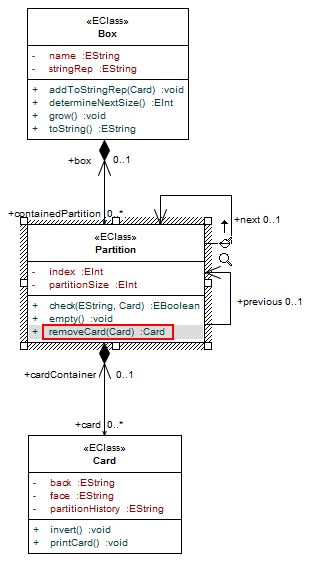
\includegraphics[width=0.6\textwidth]{ea_startSDM}
  \caption{Double-click a method to implement it}  
  \label{fig:sdm_start}
\end{center}
\end{figure}
 
\item[$\blacktriangleright$] If you did everything right, a new \emph{activity diagram} should be created and opened in a new tab with a cute anchor in
the corner, and a \emph{start node} labelled with the signature of the method (Fig.~\ref{fig:sdm_skeleton}).  

\begin{figure}[htp]
\begin{center}
 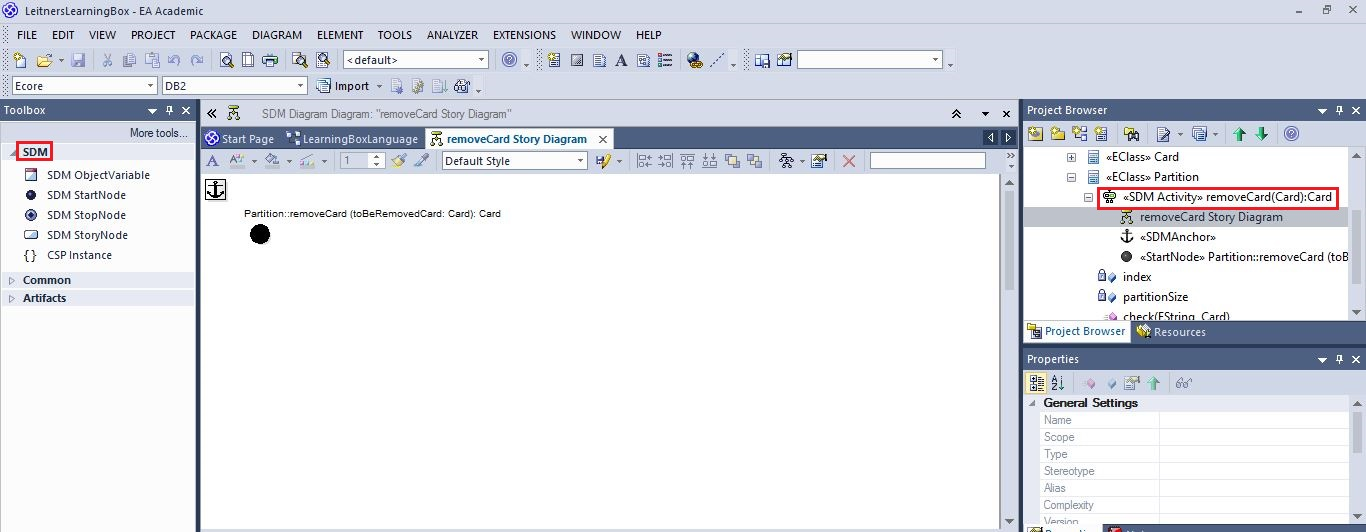
\includegraphics[width=1.0\textwidth]{ea_generatedSDM}
  \caption{Generated SDM diagram and start node}  
  \label{fig:sdm_skeleton}
\end{center}
\end{figure}

\vspace{0.5cm}

\item[$\blacktriangleright$] This diagram is where you'll model \texttt{removeCard}'s \emph{control flow}. In other words,
this is \texttt{removeCard}'s imperative top-level diagram. We refer to the whole activity diagram simply as the \emph{activity}, which always starts with a
\emph{start node,} contains \emph{activity nodes} connected via \emph{activity edges}, then finally terminates with a \emph{stop node}. Before creating
these however, let's quickly familiarise ourselves with the EA workspace.

\item[$\blacktriangleright$] First, inspect the project browser and notice that an \texttt{<<SDM Activity>>} container has been created for the method
\texttt{removeCard}. This container will eventually host every artifact related to this pattern (i.e., object variables, stop nodes, etc.). Please note
that if you're ever unhappy with an SDM, you can always delete the appropriate container in the project browser (such as this one), and start from scratch.

\item[$\blacktriangleright$] Next, note the new \texttt{SDM} toolbox that has been automatically opened for the diagram and placed to the left above
the common toolbox. This provides quick access to SDM items that you'll frequently use in your diagram. You can also invoke the active toolbox in a pop-up
context menu anywhere in the diagram by pressing the \texttt{space} bar.

\item[$\blacktriangleright$] Finally, in the top left corner of the diagram, you'll notice a small anchor. Double click on this icon to quickly jump back to the
metamodel. From there, double click the method again to jump back to the SDM. This is just a small trick to help you quickly navigate between diagrams.

\newpage

\item[$\blacktriangleright$] To begin, select the start node, and note the small black arrow that appears (Fig.~\ref{fig:sdm_quicklink}). 

\begin{figure}[htp]
\begin{center}
  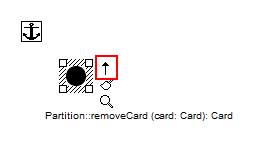
\includegraphics[width=0.5\textwidth]{ea_sdmStartNode}
  \caption{Quick link in SDM diagram to create new activity node}  
  \label{fig:sdm_quicklink}
\end{center}
\end{figure}

\item[$\blacktriangleright$] Similar to quick linking,\footnote{This was discussed in Part II, Section 2.5} a second fundamental gesture in EA is \emph{Quick
Create}.
To quick-create an element, pull the arrow and click on an empty spot in the diagram. This is basically ``quick linking'' to a non-existent element.

\item[$\blacktriangleright$] EA notices that there is nothing to quick-link to, and pops up a small, context-sensitive dialogue offering to create an element
which can be connected to the source element.

\item[$\blacktriangleright$] As illustrated in Fig.~\ref{fig:sdm_new_activity_node}, choose \texttt{Append StoryNode} to create a \emph{Story Node}.

\begin{figure}[htp]
\begin{center}
  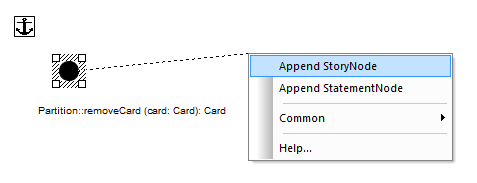
\includegraphics[width=0.8\textwidth]{ea_sdmQuickLinkStoryNode}
  \caption{Create new activity node}  
  \label{fig:sdm_new_activity_node}
\end{center}
\end{figure}

\item[$\blacktriangleright$] If you quick-created correctly, you should now have a start node, one node called \texttt{ActivityNode1}, and an edge
connecting the two items. Complete the activity by quick-creating a stop node (Fig.~\ref{fig:sdm_stop_node}).

\begin{figure}[htp]
\begin{center}
  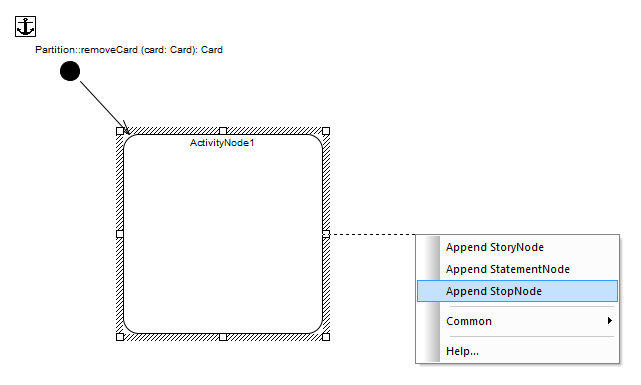
\includegraphics[width=\textwidth]{ea_sdmAppendStopNode}
  \caption{Complete the activity with a stop node}  
  \label{fig:sdm_stop_node}
\end{center}
\end{figure}

\vspace{0.5cm}

\item[$\blacktriangleright$] If everything is correct, you should now have a fully constructed activity that models the method's control flow.

\item[$\blacktriangleright$] While a \emph{stop node} is rather self explanatory, you may be wondering about the differences between the other two menu options,
the\define{Story Node}\emph{story node} and \emph{statement node}.\define{Statement Node}Since not all activity nodes can contain story patterns (e.g., start
and stop nodes), those that \emph{can} are called story nodes. Statement nodes cannot and are used instead to invoke an action, such as method execution. We'll
encounter this in a later SDM.

\item[$\blacktriangleright$] To complete this activity, double-click \texttt{ActivityNode1} to prompt the dialogue depicted in
Fig.~\ref{fig:story_pattern}. Enter \texttt{removeCardFromPartition} as the name of the story node, and select \texttt{Create this Object}.  Click
\texttt{OK}. The activity node now has a single \emph{bound} \emph{object variable}, \texttt{this}.

\item[$\blacktriangleright$] To create a new object variable, choose \texttt{SDM ObjectVariable} from the toolbox then click inside the activity node
(Fig.~\ref{fig:tool_box}). A properties window will automatically appear (Fig.~\ref{fig:object_variable_properties}).

\begin{figure}[htpb]
\begin{center} 
  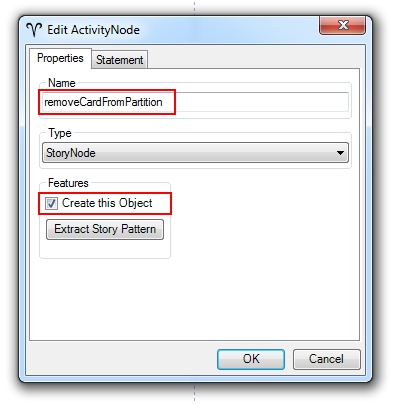
\includegraphics[width=0.6\textwidth]{ea_sdmEditActivityNode}
  \caption{Initializing a story node}  
  \label{fig:story_pattern}
\end{center}
\end{figure}

\begin{figure}[htp]
\begin{center}
  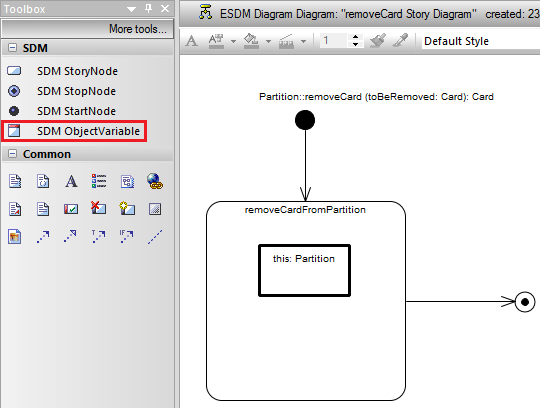
\includegraphics[width=0.8\textwidth]{ea_sdmNewObjVar}
  \caption{Add a new object variable from the toolbox}  
  \label{fig:tool_box}
\end{center}
\end{figure}

\newpage

\vspace{0.5cm}

\begin{figure}[htp]
\begin{center}
  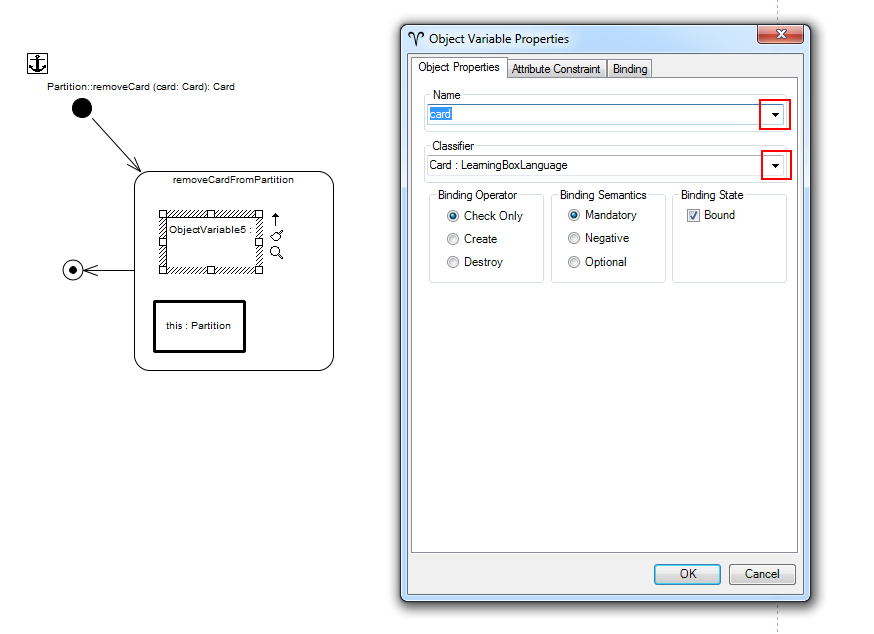
\includegraphics[width=\textwidth]{ea_sdmPropertiesObjVar}
  \caption{Specify properties of the added object variable}  
  \label{fig:object_variable_properties}
\end{center}
\end{figure}


\item[$\blacktriangleright$] Using the drop-down menus, choose \texttt{card} as the name of the object, and set \texttt{Card} as its type.
Since \texttt{card} is a parameter of the method, it is offered as a possible name which can be directly chosen to avoid annoying typing mistakes.

\item[$\blacktriangleright$] In this dialogue, note that the \texttt{Bound} option is automatically set. We have now seen two cases in this activity for bound
object variables: an assignment to \texttt{this}, and an assignment to a method parameter. Setting \texttt{card} to bound means that it will be implicitly
assigned to the parameter with the same name.

\item[$\blacktriangleright$] To create a \emph{link variable} between the current partition and the card to be removed, choose the object variable \texttt{this}
and quick link it to \texttt{card} (Fig.~\ref{fig:link_variable}).

\begin{figure}[htpb]
\begin{center}
  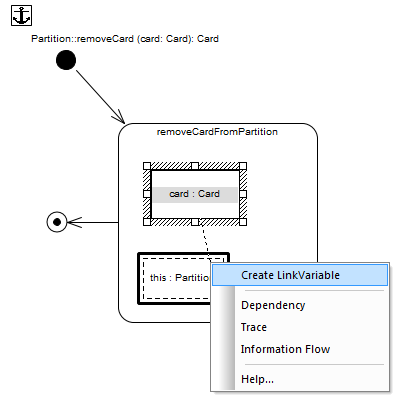
\includegraphics[width=0.6\textwidth]{ea_sdmCreateLinkVar}
  \caption{Create a link variable}   
  \label{fig:link_variable}
\end{center}
\end{figure}

\item[$\blacktriangleright$] According to the metamodel, there is only one possible link between a partition and card. Select this and set the
\emph{Binding Operator} to \texttt{Destroy} (Fig.~\ref{fig:link_variable_properties}). The reference names will automatically appear in the diagram.

\vspace{0.5cm}

% Had to force (h!) image to appear here; no other images were co-operating
\begin{figure}[h!]
\begin{center} 
 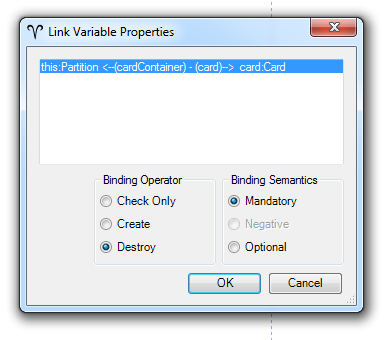
\includegraphics[width=0.6\textwidth]{ea_sdmBindLink}
  \caption{Specify properties for created link variable}  
  \label{fig:link_variable_properties}
\end{center}
\end{figure}

\vspace{0.5cm}

\item[$\blacktriangleright$] Remember how we said that this method should return the same card that was passed in? As luck would have it, a return value for an
SDM can be specified in the stop node. As depicted in Fig.~\ref{fig:stop_node_return_value}, double-click the stop node to prompt the \texttt{Edit StopNode} dialogue. 

\newpage

\begin{figure}[htbp]
\begin{center}
  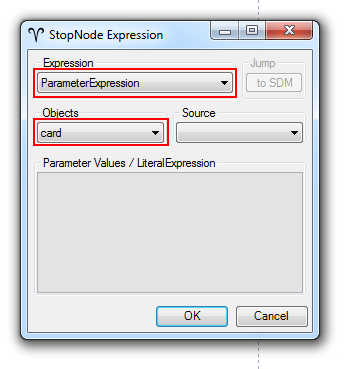
\includegraphics[width=0.5\textwidth]{ea_sdmStopNodeExpr}
  \caption{Adding a return value to the stop node}  
  \label{fig:stop_node_return_value}
\end{center}
\end{figure}

\item[$\blacktriangleright$] In the \texttt{Expression} field, choose the \texttt{ParameterExpression}\define{ParameterExpression}option.
As suggessted by its name, a \emph{ParameterExpression} is an expression that exclusively accesses method parameters. Given that \texttt{card} is the sole
parameter, the \texttt{object} will be automatically set to this value. In other words, the returned object is now implicitly \emph{bound} by having the same
name.

\vspace{0.5cm}

We're nearly done! As you can see, eMoflon uses a series of dialogues to provide a simple context-sensitive expression language for specifying  values. In the
following SDM implementations, we'll learn and discuss some other expression types eMoflon supports.

\vspace{0.5cm}

\item[$\blacktriangleright$] Returning to the activity, if you've done everything right, your first SDM should resemble
Fig.~\ref{fig:sdm_complete_control_flow}, where \texttt{removeCard}'s entire pattern layer is modeled inside the sole \emph{activity node}. The method's return
value is now indicated below the stop node.

\vspace{0.5cm}

\item[$\blacktriangleright$]  Don't forget to save your files, validate and export your pattern to the Eclipse workspace,\footnote{Go to
``\texttt{Extensions}" and select \texttt{Add-In Windows} to activate eMoflon's console. If you're unsure how to validate, export, or use this window, review
Part II, Section 3.} then build your metamodel's code from the package explorer.

\newpage

\begin{figure}[htbp]
\begin{center}
  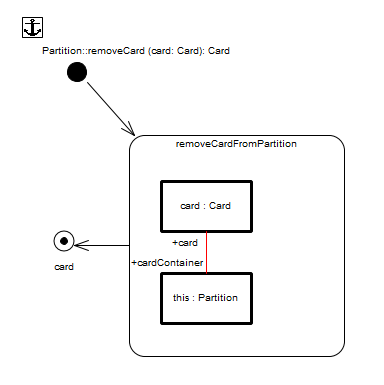
\includegraphics[width=0.7\textwidth]{ea_sdmRemoveComplete}
  \caption{Complete SDM for \texttt{Partition::removeCard}}  
  \label{fig:sdm_complete_control_flow}
\end{center}
\end{figure}

\item[$\blacktriangleright$] If you're unable to export or generate code successfully, compare your SDM carefully with Fig.~\ref{fig:sdm_complete_control_flow}
and make sure you haven't forgotten anything.

\vspace{0.5cm}

\item[$\blacktriangleright$] If you'd like to see how this SDM is implemented in the textual syntax, check out Fig.~\ref{fig:deleteReference} in the
next section.

\jumpSingle{remCard end}

\end{itemize}

